\documentclass[11pt]{article}
\pdfoutput=1
\usepackage[preprint]{acl}

\usepackage{times}
\usepackage{latexsym}
\usepackage[T1]{fontenc}
\usepackage[utf8]{inputenc}
\usepackage{microtype}
\usepackage{inconsolata}
\usepackage{hyperref}
\usepackage{url}
\usepackage{booktabs}
\usepackage{amsmath}
\usepackage{graphicx}
\graphicspath{{figures/}}
\usepackage{xcolor}
\usepackage{xspace}
\usepackage{longtable}
\usepackage{array}
\usepackage{multirow}
\usepackage[most]{tcolorbox}
\definecolor{boxframe}{RGB}{170,170,170}
\definecolor{boxtitlebg}{RGB}{208,208,208}
\tcbset{graybox/.style={
  breakable, enhanced, colback=gray!3, colframe=boxframe,
  colbacktitle=boxtitlebg, coltitle=black, fonttitle=\bfseries\small,
  arc=0.6mm, boxrule=0.4pt, left=2mm, right=2mm, top=1mm, bottom=1mm,
  before skip=3pt, after skip=3pt}}
\newtcolorbox{promptbox}[1][]{graybox, fontupper=\footnotesize\ttfamily, title={#1}}
\newcolumntype{L}[1]{>{\raggedright\arraybackslash}p{#1}}

\newcommand{\sys}{\textsc{factwash}\xspace}

% ---------------------------------------------------------------------------
% PLACEHOLDER MACRO, same discipline as paper 1: renders loud and red so a
% number that does not exist yet cannot quietly become a claim. Before any
% submission, grep for \needsdata and confirm zero hits.
% ---------------------------------------------------------------------------
\newcommand{\needsdata}[1]{\textcolor{red}{\textbf{[NEEDS DATA: #1]}}}

% Working title was "Structure Survives Compression". The two-cell experiment does not
% support that as a general claim: the effect is present on one model, absent on a
% second, and has nothing to act on at the top of the ladder. The title now says what
% was measured.
\title{Retention Fields for Agent Memory:\\
A Write Schema That Helps Where the Compressor Is Weakest}

\author{
  Alex Kwon \\
  Independent Researcher \\
  \texttt{ask@collapseindex.org}
}

\begin{document}
\maketitle

% ===========================================================================
% ABSTRACT -- write last. The claim is about COMPRESSION BEHAVIOUR, not about
% our detector. It must stand even if \sys had never been written.
% ===========================================================================
\begin{abstract}
Agent memory systems compress what they store, and compression is designed to drop
qualifiers. A natural fix is to stop writing a claim's epistemic standing as prose
(``reportedly'', ``(unconfirmed)'') and start writing it as a labelled field, on the
theory that a compressor treats prose as phrasing and a field as content. We test that
directly: $440$ matched pairs carrying identical claims and identical stance, differing
only in whether the standing is a field or a parenthetical, compressed under four levels
of budget pressure and scored by a blind reader that never sees the source or the
condition. The theory holds on exactly one of the three models we could afford to run.
On Haiku~4.5 the field form preserves standing more often ($90.0\%$ versus $81.7\%$,
McNemar $p=0.004$) and its claims are evicted from memory less often ($5$ versus $15$,
$p=0.031$). On Sonnet~4.5 the effect is absent and eviction \emph{reverses}: the bulkier
field record is the one dropped ($8$ versus $1$, $p=0.039$). On Opus~4.5 nothing is lost
in either arm, so there is nothing to prevent. We conclude that a write schema is a
real but conditional intervention, worth its cost where the compressor is weak and not
otherwise, and we report the instrument bug that made the effect look twice as large
before we caught it. Schema, deterministic field-level checker, harness and raw runs are
released.
\end{abstract}

% ===========================================================================
\section{Introduction}
% GOAL: one page. The failure is already established by prior work; this paper
% is about the FIX. Do not re-litigate detection.
% ===========================================================================

A memory system is a compressor with a database attached. It is asked to turn a
conversation into something short enough to store and retrieve, and every objective it is
tuned against, token count, latency, retrieval quality, rewards dropping words that do
not carry the answer. Hedges, attributions and dates are exactly such words.

Prior work established that this loses epistemic standing and that the loss is
consequential: a memory keeping a conclusion while dropping its basis can leave a system
worse off than no memory \citep{kwon2026reclaim}, and a hedged remark stored flat is
later obeyed as verified fact \citep{kwon2026mc}. The question this paper asks is not
whether that happens. It is what makes it stop happening.

\paragraph{The hypothesis, and what happened to it.} A compressor removes what reads as
phrasing and keeps what reads as content. Standing written into the sentence
(``reportedly'', ``(unconfirmed)'') reads as phrasing. Standing written as a labelled
field reads as content. If that is right, the fix is a write schema costing one prompt
change and no model calls:

\begin{promptbox}[the write schema]
CLAIM: <what is asserted>\\
SOURCE: <who or what it came from>\\
CERTAINTY: asserted | hedged | rumor | unverified\\
AS\_OF: <when it held>
\end{promptbox}

It is right on one model out of three. \S\ref{sec:twocell} reports the controlled test:
the field form helps on the weakest compressor, does nothing on the middle one, and has
nothing to act on at the top, where standing is not lost in either form. The useful
version of the finding is therefore conditional, and it comes with a cost we did not
anticipate: a labelled record is bulkier, and a compressor under a tight budget can
respond by evicting the whole item rather than trimming the qualifier.

\paragraph{Contributions.}
(1)~A controlled two-cell test of form, holding claim, stance, distractors and position
constant across $440$ matched pairs and four levels of compression pressure, on three
models (\S\ref{sec:twocell}). The result is positive on one, null on one, and
uninformative on the third for lack of any loss to prevent.
(2)~The eviction effect, which the survival rate hides: on one model the parenthetical
claim is dropped from memory more often, and on another the field record is
(\S\ref{sec:twocell}).
(3)~A deterministic field-level check that needs no model and no lexicon of hedged
phrasings on the memory side (\S\ref{sec:check}).
(4)~The negative results that shaped the design, including an instrument bug in our own
blind reader that inflated the headline effect until it was found
(\S\ref{sec:negatives}).

% ===========================================================================
\section{Related work}
% GOAL: 0.5 page. Compression objectives; memory systems; what prior work on
% this failure did NOT do (it detected, it did not prevent). Keep short.
% ===========================================================================
\paragraph{Memory systems compress by design.} Agent memory architectures store a
summary rather than a transcript, whether by paging between context tiers
\citep{packer2023memgpt} or by extracting standalone facts at write time
\citep{chhikara2025mem0}. Prompt compression pushes the same objective further, dropping
tokens that contribute least to reconstructing an answer
\citep{jiang2023llmlingua,wang2025recursive}. None of these objectives has a term for
epistemic standing, so a hedge is exactly the kind of token they are built to remove. Our
claim is not that these systems are careless; it is that a qualifier written as prose is
indistinguishable, to a compressor, from a qualifier written as padding.

\paragraph{Standing has long been annotated, not stored.} Hedging and speculation have a
mature annotation literature \citep{vincze2008bioscope,szarvas2012cross,farkas2010conll},
as does attribution \citep{pareti2016parc,newell2018polnear}. That work treats stance as
something to \emph{recover} from text. We take the complementary position: once a memory
system controls its own write format, stance does not have to be recovered, because it
never has to be inferred. Faithfulness benchmarks for summarisation
\citep{pagnoni2021frank,tang2023aggrefact} likewise score a summary after the fact; they
do not change what the summary is allowed to look like.

\paragraph{The detection arm.} Prior work established the failure this paper treats: a
memory that keeps a conclusion but drops its basis can leave a system worse off than no
memory at all \citep{kwon2026reclaim}, and a hedged remark stored flat is later acted on
as verified \citep{kwon2026mc}. A deterministic write-time gate for it is released and
evaluated separately. This paper is the treatment arm: not detecting the loss but
removing the conditions for it.

% ===========================================================================
\section{Where the loss happens}
\label{sec:negatives}
% GOAL: 0.75 page. The two negatives, reported first because they are what
% makes the intervention non-obvious. This is the section a reviewer respects.
% ===========================================================================

Two results shaped the design and both are negative.

\paragraph{The loss is at recording, not at compression.} We instrumented both
transitions of the same sessions: source to scratchpad note, then note to stored memory.
In $9/10$ sessions the model did record a stance cue in its note, and of those, the cue
was still recoverable after compression in most cases. The intermediate note is
stance-\emph{preserving}: what a model writes down explicitly tends to survive
consolidation, and the leak is upstream of the compressor. We report this as a pilot and
lean nothing on the exact counts, because the automatic scorer we used for it counts
cue \emph{tokens}, and compression frequently reworded a hedge rather than deleting it
(``(unconfirmed)'' became ``pending confirmation''), which that scorer records as a loss.
The open-class problem ate the measuring instrument inside a probe about the open-class
problem. $n=10$, one model.

\paragraph{Repairing the prose does not survive.} Gating the note and asking the model to
restore what it dropped produces a clean null end to end:
the repair fired on $8/10$ notes, cost $23.4\%$ more input tokens, and changed the final
verdict on zero of them, $0$ recovered and $0$ broken. The repair is not ignored; it is undone. The model
restores standing as a parenthetical (``(per informal report)'') and the compressor
removes it, which is what a compressor is for. This is the observation the rest of the
paper turns into a design.

\paragraph{A third negative, in our own instrument.}
\label{sec:instrument}
The blind reader was asked for JSON. When a stored memory carried \emph{two} stance cues
it reliably emitted this:

\begin{promptbox}[what the judge actually returned]
\{"presented\_as": "qualified", "cue": "may have", "unconfirmed rumor from third party"\}
\end{promptbox}

which is not valid JSON. \texttt{json.loads} raised, the verdict was recorded as null,
and the scorer counted it as ``standing did not survive''. The instrument was discarding
its own clearest positives, and discarding them precisely on the memories with the most
surviving stance. It affected $6\%$ of trials. Because those trials were the
unambiguous ones, and because the parenthetical arm produced more of them, the bug
inflated the headline: on the affected data the pooled advantage read
$+9.3$ points, and after the fix the same design gives $+4.0$. We report this because
the direction is the instructive part. A measurement error in a paper's own scorer is
not a coin flip; it lands where the scorer is fragile, and a scorer is usually most
fragile on the cases its author considered obvious. The harness now stores every raw
judge reply and reports what fraction needed the fallback parser ($29/880$, with none
unusable), so the next failure of this kind is visible in the data rather than absorbed
by it.

% ===========================================================================
\section{Field versus prose, held constant}
\label{sec:twocell}
% GOAL: 1 page + table. THE CORE EXPERIMENT. Same claim, same stance, same
% compressor, one variable: the FORM the stance is written in.
% ===========================================================================

The observation above is post hoc: the notes that happened to use fields differed from
the notes that happened to use parentheticals in more than form. This section removes
that confound.

\paragraph{Design.} Ten claims are each written twice, carrying the \emph{identical}
assertion and the \emph{identical} stance content, differing only in where the standing
sits:

\begin{promptbox}[the two cells]
\textbf{field}\quad Alice has admin access\\
\phantom{\textbf{field}}\quad SOURCE: a third party\\
\phantom{\textbf{field}}\quad CERTAINTY: rumor\\[2pt]
\textbf{paren}\quad Alice has admin access (per a third party; rumor, unconfirmed)
\end{promptbox}

Both go to the same compressor with the same prompt, settings and temperature. Pairing is
strict: for a given (claim, pressure, replicate) the two arms receive the same filler
notes in the same positions, drawn from a seed that does not depend on the arm, so
nothing but form differs.

\paragraph{Pressure is a factor, not a nuisance.} A first version of this experiment
compressed a single one-sentence note and returned a clean null, for the good reason that
it did not compress: the input averaged $60$ characters and the stored memory came out at
$90$. Nothing was dropped because nothing had to be. Budget pressure is therefore swept:
\textsc{none} ($1$ note, ``one or two sentences''), \textsc{low} ($6$ notes, one line
each), \textsc{high} ($6$ notes, $40$ words total) and \textsc{extreme} ($6$ notes, eight
words per line).

\paragraph{Readout.} A separate model sees only the stored memory and the claim to look
up, never the source note, the arm, or the pressure level, and answers whether the claim
is stored as established fact, as qualified, or is absent. Judge replies are parsed
without requiring valid JSON, for reasons given in \S\ref{sec:instrument}.

\paragraph{Result.} Figure~\ref{fig:twocell} and Table~\ref{tab:twocell}. The hypothesis
holds on one model of three.

\begin{figure*}[t]
\centering
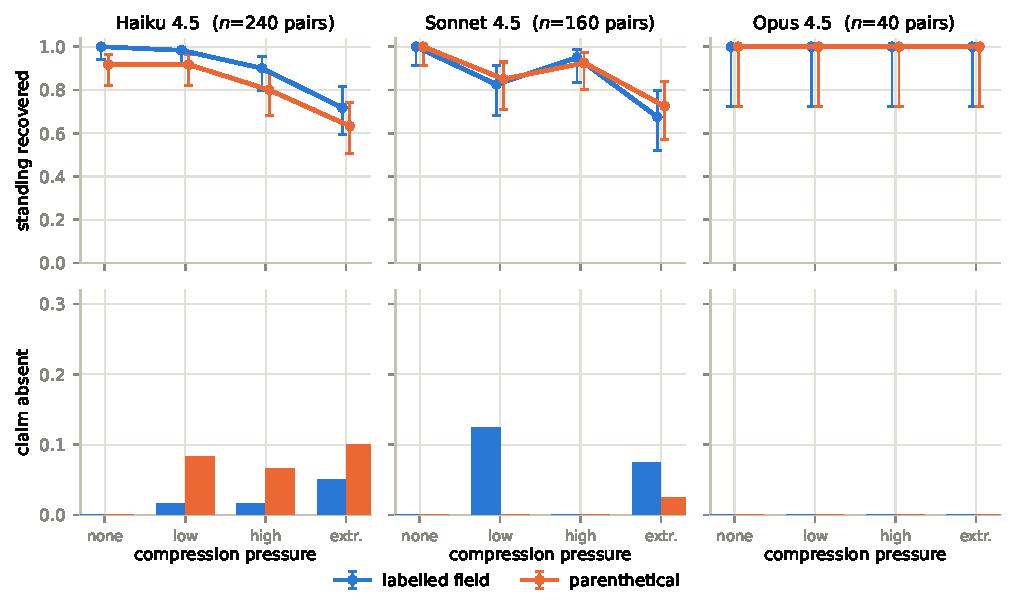
\includegraphics[width=\textwidth]{fig_twocell.pdf}
\caption{Two-cell result by model. \textbf{Top:} share of stored memories from which a
blind reader can still recover the claim's standing, by compression pressure, with
$95\%$ Wilson intervals. \textbf{Bottom:} share where the claim is absent from the stored
memory altogether. The field advantage is present on Haiku, absent on Sonnet, and
unmeasurable on Opus, which loses no standing in either arm at any pressure we applied.
Eviction runs the opposite way on Sonnet from the way it runs on Haiku.}
\label{fig:twocell}
\end{figure*}

\begin{table}[t]
\centering\small
\begin{tabular}{@{}l r r r r@{}}
\toprule
Model & pairs & field & paren & McNemar $p$ \\
\midrule
Haiku 4.5  & 240 & $90.0\%$ & $81.7\%$ & $0.004$ \\
Sonnet 4.5 & 160 & $86.3\%$ & $87.5\%$ & $0.82$ \\
Opus 4.5   & 40  & $100\%$  & $100\%$  & --- \\
\bottomrule
\end{tabular}
\caption{Standing recovered by a blind reader, pooled over the four pressure levels.
Opus loses no standing in either arm, so the comparison is undefined rather than null.
The Opus run is a single complete replicate: the API budget ran out mid-run, and the
incomplete replicate is excluded rather than averaged in.}
\label{tab:twocell}
\end{table}

On \textbf{Haiku 4.5} the field form preserves standing in $216/240$ pairs against
$196/240$ for the parenthetical, a paired advantage of $32$ discordant pairs to $12$
(exact McNemar $p = 0.004$). The gap is present at every pressure level and does not
widen with pressure, which contradicts the prediction we recorded in the harness before
running it: we expected no difference at \textsc{none} and a widening advantage as the
budget tightened. Neither half held. The advantage is already present at \textsc{none}
($100\%$ versus $91.7\%$) and is no larger at \textsc{extreme} ($71.7\%$ versus
$63.3\%$) than at \textsc{high}.

On \textbf{Sonnet 4.5} the effect is absent: $138/160$ against $140/160$, discordant
pairs $9$ to $11$, $p = 0.82$. The point estimate is slightly negative. On
\textbf{Opus 4.5} both arms recover standing in $40/40$ pairs at every pressure level,
including eight words per line. There is no loss for the schema to prevent, so the model
is uninformative about the mechanism rather than evidence against it.

\paragraph{Eviction, and a cost we did not anticipate.} Survival rate hides a second
outcome: the claim can be dropped from the digest entirely. It is not rare and it is not
symmetric. On Haiku the parenthetical claim is evicted $15$ times against the field's
$5$ ($p = 0.031$), which compounds the field advantage: the parenthetical note is both
more likely to lose its standing and more likely to lose the whole claim. On Sonnet the
asymmetry reverses and is also significant, $8$ field evictions against $1$
($p = 0.039$). The plausible reading is that a multi-line labelled record costs more
budget than a parenthetical, so a compressor good enough to keep stance either way will
sometimes drop the bulkier item instead of trimming it. If that is right, the schema
trades a stance-fidelity gain for a retention risk, and which way the trade goes depends
on the compressor.

\paragraph{What we would need to settle it.} Three models from one family is a ladder,
not a sample, and the two informative points disagree. The reading we favour, that the
schema pays where the compressor is weak and is redundant where it is strong, is
consistent with all three but is not established by them: an equally consistent reading
is that Haiku is the outlier. Separating those needs models from other families and a
pressure regime severe enough to make Opus lose something, neither of which the
API budget for this paper reached.

% ===========================================================================
\section{The schema end to end}
\label{sec:endtoend}
% GOAL: 1 page. Does it hold in a pipeline, and on a real memory system?
% ===========================================================================
The two-cell experiment isolates form. It does not tell us whether a model asked to
\emph{use} the schema does so well enough for the isolated effect to appear in a
pipeline. A pilot suggests it can, on the same model where the two-cell effect was
found: writing the note to the schema and then compressing to ordinary prose raised
clean writes from $3/10$ to $7/10$, and when the model filled the schema it filled it
completely, keeping all four fields in $10/10$ records. It classified $8/10$ sources as
something other than plainly asserted ($6$ rumor, $2$ hedged), so the recording step
works. This is $n=10$ on one model and is a pilot, not a result.

\paragraph{Independent readout.} The pilot above is scored by a deterministic checker we
also wrote, which is not an independent judge of our own intervention. The two-cell
experiment therefore uses a different readout entirely: a model that sees only the stored
memory and the claim to look up, never the source, the arm, or the pressure level. That
is the readout every number in \S\ref{sec:twocell} comes from, and it is the reason we
trust the null on Sonnet as much as the positive on Haiku.

% ===========================================================================
\section{Checking a record}
\label{sec:check}
% GOAL: 0.5 page. The checker, and the argument that structure removes the
% HARD half of the detection problem.
% ===========================================================================

Once standing is a field, checking it stops needing a model. The hard half of detection
is recognising stance in a rewrite, an open-class problem with no finite vocabulary. A
field does not need recognising. The released check compares the record against the
source with three rules: if the source hedges, \texttt{CERTAINTY} may not read
\texttt{asserted}; if the source names a speaker, \texttt{SOURCE} may not be empty; if
the source dates the claim, \texttt{AS\_OF} may not be empty. A record missing its
retention fields is \textsc{malformed}, never a pass.

\paragraph{An instrument note.} A prose detector scores a schema memory
\emph{worse} than a prose memory, because \texttt{CERTAINTY: hedged} preserves the
standing perfectly and contains no word a hedge lexicon knows.
Measured: a schema note compressed into a schema memory scored $5/10$ clean under the
prose detector against $7/10$ for the same schema note compressed into prose, an
apparent regression that is entirely an artefact of the instrument. Inspection of the
records showed all four fields intact in $10/10$ cases. The record is more
machine-readable, not less; it has to be read as a record.

% ===========================================================================
\section{Limits}
% ===========================================================================
\paragraph{The schema costs bulk, and bulk is what a compressor spends.} This is the
concrete form of the Sonnet eviction result. A four-field record is several lines where a
parenthetical is a clause, and under a hard budget the compressor has to put that
somewhere. Trimming the qualifier is one option; dropping the whole item is another, and
we observed the second.

\paragraph{A filled field can be wrong.} Every failure we measure is a field being
\emph{dropped}. A field confidently filled with the wrong value, \texttt{CERTAINTY:
asserted} on a rumour, is a worse failure and is invisible to a checker that only asks
whether the field is present. Our checker catches the subset where the source's own
hedging is detectable; it cannot catch a misfilled field whose source reads plainly.

\paragraph{The schema is English and the lexicons are English.} Detecting stance in the
\emph{source} still uses deterministic lexicons, and every open-class limit documented
for the prose gate applies to that half unchanged. What the schema removes is the second
half of the problem, recognising stance in the rewrite.

\section{Conclusion}

The idea is appealing enough that we expected it to be true in general: write a claim's
standing as structure and a compressor will treat it as content rather than as phrasing.
Held constant across $440$ matched pairs, it is true on one model, absent on another, and
untestable on a third that loses no standing to begin with. The useful statement is
conditional. A write schema is worth its cost where the compressor is weak enough to
drop qualifiers, which describes the small fast models that agent memory pipelines
actually run at the write step, and it is redundant where the compressor is strong. It
is not free: on one model the labelled record was the one evicted under pressure.

We would rather ship that than the general claim. The two negatives that shaped this work
were both more informative than the positive result we were looking for at the time: the
loss turned out to be at recording rather than at compression, and repairing prose after
the fact turned out to be perfectly undone by the next compression step. The third
negative was in our own scorer, and it was inflating our headline by a factor of two
until we looked at why it was silently discarding verdicts.

\section*{Limitations}

Three models from a single family is a ladder, not a sample, and the two informative
points disagree with each other. We favour the reading that the schema pays where the
compressor is weak, but ``Haiku is the outlier'' fits the same three points, and
distinguishing them needs models from other families. The Opus arm is a single complete
replicate, $n=40$ pairs: the API budget ran out mid-run, and rather than average an
unbalanced replicate we dropped it and report the drop. Our pressure manipulation tops
out below what a frontier compressor finds difficult, which is why Opus is at ceiling,
so we cannot say whether the effect would appear there under a harder budget.

The stimuli are ten hand-written English claims in an office-work register, with
stance-free fillers, chosen so that the two arms could be exactly matched. That control
is what makes the comparison clean and is also what makes it artificial: real notes are
not matched pairs. The end-to-end pilot ($n=10$, one model) is reported as a pilot and
nothing in the conclusion rests on it. Finally, ``standing recovered'' is one model's
judgement of another model's output. It is blind to the condition, which is the property
we needed, but it is not a human annotation and we did not collect one.

\section*{Ethics Statement}

All stimuli are synthetic, written by the authors for this experiment. They describe
fictional colleagues and fictional internal facts, contain no personal data, and were not
drawn from any real correspondence. The failure this work addresses is one where a system
overstates its confidence to its own operator; the intervention is a change to how a
system records what it was told, and we see no dual-use concern in releasing it. Raw runs
including every model output are released alongside the code so the analysis can be
checked rather than taken on trust.

\bibliography{references}

\appendix
\clearpage
\onecolumn

\section{Claims and evidence}
\label{app:claims}

Every load-bearing claim, its evidence, and its status. Rows marked \textsc{pending} are
what this draft still owes.

\medskip
{\small
\begin{longtable}{@{}L{0.44\textwidth} L{0.18\textwidth} L{0.30\textwidth}@{}}
\toprule
\textbf{Claim} & \textbf{Evidence} & \textbf{Status} \\
\midrule
\endfirsthead
\toprule
\textbf{Claim} & \textbf{Evidence} & \textbf{Status} \\
\midrule
\endhead
\bottomrule
\endlastfoot

Stance written as a field survives compression more often than the same stance written as
prose. & \S\ref{sec:twocell}, Fig.~\ref{fig:twocell} & \textsc{shown on one model of
three}: Haiku $90.0\%$ vs $81.7\%$, $p=0.004$, $n=240$ pairs. Sonnet null
($p=0.82$). Opus loses nothing in either arm, so undefined \\

\textbf{Stance written as a field survives compression more often, as a general property
of compressors.} & \S\ref{sec:twocell} & \textsc{not shown}: this is the claim the
working title made and the data does not support it. Two informative models disagree \\

The advantage widens as compression pressure increases. & \S\ref{sec:twocell} &
\textsc{retracted}: predicted in the harness before the run, not observed. On Haiku the
gap is already present at zero pressure and no larger at the extreme \\

The schema is free of retention cost. & \S\ref{sec:twocell} & \textsc{not shown}: on
Sonnet the field record is evicted from memory \emph{more} often than the parenthetical
($8$ vs $1$, $p=0.039$) \\

A write schema raises the share of memory writes that retain standing. &
\S\ref{sec:endtoend} & \textsc{pending}: pilot $3/10 \to 7/10$, one model, one prompt
set, $n=10$ \\

The loss occurs at recording rather than at compression. & \S\ref{sec:negatives} &
\textsc{pending}: pilot $9/10$ vs $1/10$ on one model \\

Our blind reader measured what we thought it measured. & \S\ref{sec:instrument} &
\textsc{not shown for the first runs}: a parser bug discarded $6\%$ of verdicts,
non-randomly, and inflated the effect from $+4.0$ to $+9.3$ points. Fixed, re-run, and
the pre-fix data is archived rather than pooled \\

Repairing the note in prose fixes the stored memory. & \S\ref{sec:negatives} &
\textsc{not shown}: clean null in the pilot, $0$ recovered and $0$ broken \\

Field-level checking needs no model on the memory side. & \S\ref{sec:check} &
\textsc{shown} by construction; the released checker uses no model \\

\textbf{This paper's detector is an independent judge of this paper's intervention.} &
\S\ref{sec:endtoend} & \textsc{not claimed}: it is our own gate, which is why a second
readout is required \\

\end{longtable}
}

\end{document}
